\documentclass{article}
\usepackage{graphicx}
\usepackage{blindtext}
\usepackage[T1]{fontenc}
\usepackage[utf8]{inputenc}
\usepackage{mathtools}
\usepackage{amssymb}
\usepackage{amsmath}
\usepackage{gensymb}
\usepackage{url}
\usepackage{float}
\usepackage{fancyhdr}
\usepackage[a4paper,left=3cm,right=3cm,top=2cm,bottom=4cm,bindingoffset=5mm]{geometry}
\usepackage{etoolbox}%
\usepackage[ngerman]{babel}

\newcommand{\makefootnotelist}[1]{%
	\parbox{0.8\textwidth} {%
		\footnotesize{%
			\renewcommand*{\do}[1]{##1\\}%
			\dolistcsloop{#1}}}}%
\newcommand{\fancyfootnote}[1]{%
	\footnotemark{}%
	\def\listname{footlist\thepage}%
	\def\n{$^{\the\numexpr\value{footnote}}$}
	\ifcsdef{\listname}%
	{\listcseadd{\listname}{\n\ #1}}%
	{\csedef{\listname}{}%
		\listcseadd{\listname}{\n\ #1}}%
	\fancypagestyle{fancyfootnote}{%
		\fancyfoot[LO,RE]{\makefootnotelist{\listname}}%
		\fancyfoot[RO,LE]{Page \thepage}%
		\fancyfoot[C]{}%
	}\thispagestyle{fancyfootnote}}%


\pagestyle{fancy}
\fancyhf{}
\rhead{\leftmark}
\lhead{B3.1}
\rfoot{Page \thepage}
\renewcommand{\footrulewidth}{0.2pt}


\title{Praktikumsbericht B 3.2: \\ \underline{$\gamma$-Spektroskopie mit HPGe-Detektor}}
\author{Alexander Obradovic\\
		\texttt{7338968}
		\and
		Marcus Sickmöller\\
		\texttt{7359786}
		\and
		Tom Sittig\\
		\texttt{7345424}}
\date{04.06.2021}

\begin{document}
	\maketitle
	\begin{center}
	
\includegraphics[scale=0.13]{siegel.jpg}
	\end{center}
	
	\newpage
	\tableofcontents
	\newpage
	\section{Einführung}
	\newpage
	\section{Vorbereitung}
	\begin{itemize}
	\item \textbf{Was bedeutet der Wirkungsquerschnitt anschaulich?}\\\\
	Der Wirkungsquerschnitt $\sigma$ ist eine Angabe für die Wahrscheinlichkeit, dass eine bestimmte mögliche Interaktion stattfindet. Von welchen Größen, in welcher Kapazität der Wirkungsquerschnitt explizit abhängt unterscheidet demnach, welchen Vorgang man beobachtet/beschreibt. Im Falle unseres Experiments sind alle drei Wirkungsquerschnitte $\sigma_{Photo,Compton,Paar}$ abhängig von der Energie des Photons $E_\gamma$ und der Ordnungszahl $Z$.\\
	Der Wirkungsquerschnitt ist in der Dimension Fläche gegeben und wird in der Kernphysik standardmäßig in Barn angegeben ($1b=10^{-28}m^2$).
	   
	\item \textbf{Wie hängen die Wirkungsquerschnitte von der Ordnungszahl \boldmath$Z$ und Photonenenergie \boldmath$E_\gamma$ ab?}\\\\
	Der Wirkungsquerschnitt des Photons $\sigma_\gamma$ ist zusammengesetzt aus den Wirkungsquerschnitten der einzelnen, möglichen Interaktionen, also eben dem Photo- und Compton-Effekt, sowie der Paarbildung. $\sigma_\gamma=\sigma_{Photo}+\sigma_{Compton}+\sigma_{Paar}$. \\
	Der Wirkungsquerschnitt des Photoeffekts ist gegeben durch die Formel 
	\begin{equation}
	\sigma_{Photo}\approx3\cdot10^{12}\frac{Z^5}{E_\gamma^{3.5}}
	\end{equation}
	Der des Comptoneffekts ist gegeben durch die Klein-Nishina Gleichung, welche einen linearen Zusammenhang $\sigma_{Compton}\propto Z$ herstellt. Zudem ist sie abhängig von dem Quotient $k=E_\gamma/E_e$.\\
	Der Wirkungsquerschnitt der Paarbildung wird beschrieben durch die Maximon Gleichung, welche ebenfalls eine Abhängigkeit vom Term $k$ besitzt, sowie $\sigma_{Paar}\propto Z^2$.\\
	Trägt man den Wirkungsquerschnitt $\sigma_\gamma$ gegen die Energie des Photons $E_\gamma$, so erhält einen Graphen folgender Form\fancyfootnote{Ertley, Camden. (2014). STUDYING THE POLARIZATION OF HARD X-RAY SOLAR FLARES WITH THE GAMMA RAY POLARIMETER EXPERIMENT (GRAPE)}
	\begin{figure}[h!]
		\centering
		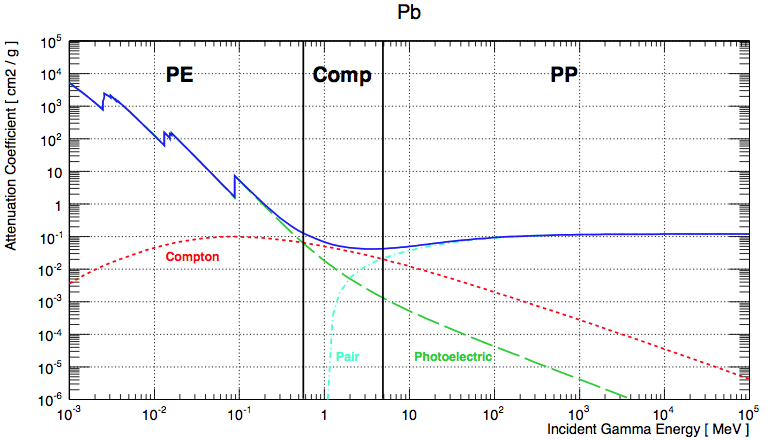
\includegraphics[scale=0.6]{crosssection.jpg}
		\caption{Wirkungsquerschnitt, hier $Z=82$}
	\end{figure}
	
	\item \textbf{Wie hängt beim Comptoneffekt die Energie des Photons von dem Streuwinkel \boldmath$\vartheta$ ab?}\\\\
	Das Photon erfährst eine Energieänderung $\Delta E$ in Abhängigkeit vom Streuwinkel nach dem Zusammenhang $\Delta E=\frac{m_ec^2}{(1-cos(\vartheta))}$, wobei die Energie $\Delta E$ an das Elektron übertragen wird.
	\item \textbf{Warum ist eine Paarbildung erst ab \boldmath$E_\gamma\geq1022keV$ zu beobachten?}\\\\
	Bei der Paarbildung wird ein Elektron-Positron-Paar erzeugt. Beide Teilchen besitzen eine Masse $m_e$ deren Erzeugung Energie nach dem Zusammenhang $E=2\cdot(m_ec^2)=1.022MeV$ erfordert.  
	\item \textbf{Welche physikalischen Hintergründe haben die in der Abbildung [Abb. 2] auftretenden Strukturen?}\\\\
	\begin{figure}[h!]
	\centering
	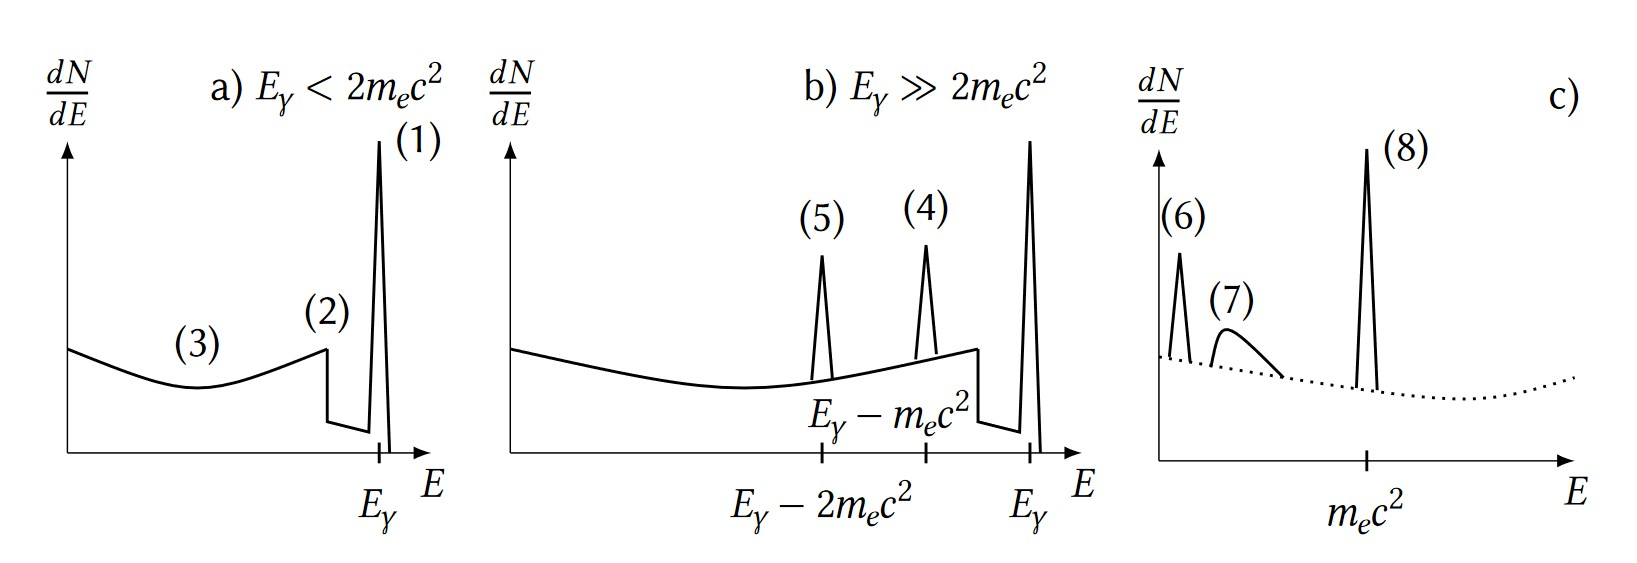
\includegraphics[scale=0.4]{Abb1.jpg}
	\caption{Schematisches $\gamma$-Spektrum}
	\end{figure}
	\begin{enumerate}
		\item Die gesamte Energie des Photons wird auf ein Elektron des Germanium Atoms übertragen, welches aus seiner Schale gelöst wird, weshalb sich der Peak auch bei $E=E_\gamma$ befindet.
		\item Die Compton-Kante ist ein scharfer Cutoff, da die maximale durch den Comptoneffekt übertragene Energie bei $\vartheta=180\degree$ frei wird.
		\item Der Compton-Untergrund ist die Energie die durch den Comptoneffekt an ein Elektron übertragen wird. Der Streuwinkel ist hier entscheidend für den Anteil der Energie, die abgegeben wird.
		\item Der Single-Escape-Peak entsteht, da bei der Paarbildung eines der entstandenen Teilchen sich mit einem anderen annihiliert und das so erzeugte Photon mit $511keV$ nicht von dem Detektor manchmal nicht erfasst wird.
		\item Der Double-Escape-Peak entsteht aus selbigen Grund wie der Single-Escape-Peak, jedoch werden das bei beiden Annihilationen erzeugte Photon, mit je $511keV$, nicht erfasst.
		\item Die Röntgenpeaks sind die charakteristische Röntgenstrahlung, die durch Anregung eines Elektrons in eine höhere Schale, und deren subsequenten Abfall auf eine tiefere erzeugt werden. 
		\item Wenn das Photon außerhalb des Detektors durch den Comptoneffekt zurück in diesen gestreut wird, nun mit geringerer Energie, kann es dort seine restliche Energie durch den Photoeffekt abgeben, womit ein weiterer, kontinuierlicher Rückstreu-Peak entsteht. 
		\item Der Annihilations-Peak entsteht durch die Vernichtung eines Teilchens, das bei der Paarbildung entstanden ist. Ein Photon mit der Masse-Energie des Teilchens, $511keV$, wird emittiert und detektiert.     
	\end{enumerate}
	\item \textbf{Was geschieht beim Zusammenführen eines p- und eines n-Kontakts?}\\\\
	Wird ein n-dotierter Kristall mit einem p-dotierten zusammen entsteht ein p-n-Übergang. Zwischen den beiden Kristallen entsteht eine „Verarmungszone“, durch die Diffusion der Ladungsträger. Diffusion der Ladungsträger beschreibt den Prozess, bei dem die beiden dotierten Kristalle versuchen die Ladungsunterschiede auszugleichen dabei werden nicht ausgleichbare unbewegliche Verunreinigungen erzeugt die man als Dotierung bezeichnet. In der Nähe der Verbindungsstelle kommen diese am häufigsten vor. \\
	Die Verarmungszone bildet das aktive Detektionsvolumen. Durch Anlegen einer Spannung von außen, kann das Detektionsvolumen vergrößert werden. So kann die Detektionseffizienz erhöht werden.
	\item \textbf{Warum wird der Detektor in Sperrrichtung betrieben?}\\\\
	Durch das Anlegen der Spannung in Sperrrichtung steuert man, dass sich die Verarmungszone über den p-dotierten Kristall ausbreitet. Dies wird getan, da es eine einfache Möglichkeit ist hochreine Kristalle nur sehr leicht zu dotieren und an diesen leicht dotierten Kristall zwei stark dotierte Kristalle zu setzen. Diese Methode wird als p-i-n Diode bezeichnet, wobei das i den leicht dotierten hochreichen Kristall bezeichnet.
	So kann eine sehr viel höhere Detektor Genauigkeit erzeugt werden.
	\item \textbf{Wozu dient die gesamte Elektronik?}\\\\
	Mit der Messelektronik werden ausgesendete $\gamma$-Quanten registriert, indem das $\gamma$-Quant im aktiven Volumen wechselwirkt und somit Compton-Streuung, Photoeffekt oder Paarbildung entsteht (je nach Energie des $\gamma$-Quants)
	\item \textbf{Welche Funktion haben Hoch- und Tiefpass?}\\\\
	Die Hauptfunktion von Hoch- und Tiefpass ist nur hohe beziehungsweise tiefe Frequenzen durchzulassen, die über beziehungsweise unter einer Grenzfrequenz liegen. Das Signal wird eindeutiger, da Störfrequenzen herausgefiltert werden.
	\item \textbf{Was ist ein FET und warum kann man damit Signale verstärken?}\\\\
	Ein FET (Feldeffekttransistor) ist eine Art von Transistor der über spannungsgesteuerte Schaltungselemente betrieben wird. der dazu genutzt wird, um Signale zu verstärken. Das Signal kann damit verstärkt werden in dem eine hohe konstante Quellspannung angelegt wird, die am Transistor gesperrt wird, solange keine Spannung am Gate anliegt. Der Detektor (p-n-Diode) ist am Gate angeschlossen, somit wird das Gate geöffnet so bald ein $gamma$-Quant registriert wird. Da die Quellenspannung manuell eingestellt werden kann, ist es einfach so das Signal zu verstärken.
	\item \textbf{Wozu wird die Pole-Zero-Einstellung benötigt?}\\\\
	Mithilfe der Pole-Zero-Einstellung können Unter- und Überschwinger nach dem Hauptverstärker korrigiert werden.
	\item \textbf{Welcher Detektor hat die bessere intrinsische Auflösung, ein Germanium oder ein Siliziumdetektor?}\\\\
	Die intrinsische Effizienz bestimmt gemeinsam mit der geometrischen Effizienz den Nachweiseffizienz Faktor $\epsilon$. Die intrinsische Auflösung wird durch Materialeigenschaften, Größe des aktiven Detektionsvolumen und dessen Energie bestimmt. Da Germanium eine höhere Ordnungszahl und eine höhere Dichte hat ist die Nachweiswahrscheinlichkeit höher als bei Siliziumdetektoren.
	\item \textbf{Was geschieht beim Trapping?}\\\\
	Das Trapping beschreibt den Ladungsträgerverlust durch tiefe Oberflächenstörstellen.
	\item \textbf{Nimmt die Full-Energy-Peak-Effizienz mit zunehmender Energie zu oder ab? Worauf ist dies zurückzuführen?}\\\\
	Die Full-Energy-Peak-Effizienz ist bei höherer Energie geringer, da es häufiger zu Paarbildung bei hoher Energie kommt.
	
	\end{itemize}
\end{document}